\documentclass[12pt]{article}


\usepackage[dvips,letterpaper,margin=0.75in,bottom=0.5in]{geometry}
\usepackage{cite}
\usepackage{slashed}
\usepackage{graphicx}
\usepackage{amsmath}
\usepackage{braket}
\usepackage{exercise}
\usepackage{feynman}

\DeclareMathOperator{\Tr}{Tr}
\newcommand{\gv} {\ensuremath{g_{\mathrm v}}}
\newcommand{\ga} {\ensuremath{g_{\mathrm a}}}
\newcommand{\Ps} {\ensuremath{\slashed{P}}}
\newcommand{\Qs} {\ensuremath{\slashed{Q}}}
\newcommand{\Rs} {\ensuremath{\slashed{R}}}
\newcommand{\Ss} {\ensuremath{\slashed{S}}}
\newcommand{\ps}{\ensuremath{\slashed{p}}}
\newcommand{\GeV} {\ensuremath{\mathrm{Ge\kern -0.08em V}}}

\begin{document}

\title{Standard Model Cross Sections \\ for Electron-Positron Annihilation}
\author{Michael Mulhearn}

\maketitle
\section{Introduction}
The purpose of this note is to directly connect the Standard Model Theory, as typically taught at the graduate level for students in both theoretical and experimental particle physics, with the state-of-art software used to calculate cross-sections and Monte Carlo data samples.  We start with a guided tour through the standard model cross-section calculation for $e^+e^- \to \mu^+\mu^-$ at $Q^2$ much larger than the muon mass, and then reproduces these findings using MadGraph.  A familiarity with the Feynman rules for the Standard Model is presumed, as available in the Appendix of {\bf An Introduction to Quantum Field Theory} by Peskin and Shroeder.  No prior experience with Madgraph is assumed, although familiarity with ROOT, or an alternative, is assumed for the computing exercises.  Note that the Appendix contains all of the physical constants needed to complete the exercises.

\section{Matrix Elements}

\begin{figure}[htbp]
\begin{center}
\begin{feynman}
    \fermion{1.00, 1.00}{0.0, 0.2}
    \fermion{0.0, 1.8}{1.00, 1.00}
    \electroweak{1.00, 1.00}{2.00, 1.00}
    \fermion{3.00, 0.2}{2.00, 1.00}
    \fermion{2.00, 1.00}{3.00, 1.8}
    \node at (0,0) {$\bar{v} \equiv \bar{v}^{r_2}(p_2)$};
    \node at (0,2) {$u \equiv u^{r_1}(p_1)$};
    \node at (3,2) {$\bar{w} \equiv \bar{w}^{s_1}(p_3)$};
    \node at (3,0) {$x \equiv v^{s_2}(p_4)$};
    \node at (1.5,1.2) {$Z/\gamma$};
    \node at (1.5,0.8) {$k = p_1 + p_2$};
    \node at (0,0.4) {$e^+$};
    \node at (0,1.6) {$e^-$};
    \node at (3.0,0.4) {$\mu^+$};
    \node at (3.0,1.6) {$\mu^-$};
\end{feynman}
\caption{\label{fig:feyn} Feynman diagram for the process $e^- e^+ \to Z/\gamma \to \mu^- \mu+$ and the definition of the four spinors: $u$,$v$,$w$, and $x$.  Don't stress yourself writing $u^{r_1}(p_1)$ a million times!}
\end{center}
\end{figure}

\begin{Exercise}
For spinors $u$ and $\bar{v}$ defined as in Fig.~\ref{fig:feyn} with $k = p_1 + p_2$ show that:
\begin{equation}
  \left( \bar{v} \gamma_\mu u \right) k^\mu = 0 \label{eqn:kvanishes}
\end{equation}
as a result of the Dirac Equation for the spinors $u$ and $\bar{v}$:
\begin{eqnarray*}
(\ps-m)  u(p) &=&  0 \\
(\ps+m) v(p) &=&  0
\end{eqnarray*}
\end{Exercise}

\begin{Exercise}
Following the conventions in Fig.~\ref{fig:feyn}, and making use of Equation~\ref{eqn:kvanishes}, show that the Feynman rules for the $\gamma$ and $Z$ processes result in the following two matrix elements:
\begin{eqnarray}
\mathcal{M}_\gamma &=&  \frac{ie^2}{Q^2} \left( \bar{w} \gamma^\mu x \right) \left( \bar{v} \gamma_\mu u \right) \label{eqn:mg}\\ 
\mathcal{M}_Z &=& \frac{ig^2}{4\cos^2\theta_W}\; \frac{1}{Q^2-m_Z^2 + i \epsilon} \; \left\{ \bar{w} \gamma^\mu  (\gv-\ga\gamma_5) x \right\} \left\{ \bar{v} \gamma_\mu (\gv-\ga\gamma_5) u \right\} \label{eqn:mz}
\end{eqnarray}
\end{Exercise}

\section{Preliminary Calculations}

Both matrix elements in Equations~\ref{eqn:mg} and \ref{eqn:mz} consist of products of bilinear forms which have the same form:
\begin{equation*}
\mathcal{M}_A = C_A \, (\bar{w} \, A^\mu \, x) (\bar{v} \, A_\mu \, u) 
\end{equation*}
where $A^\mu$ is a product of gamma matrices and $C_A$ is a complex valued function of kinematic variables.  Noting that:
\begin{eqnarray*}
(\bar{v} X u)^\dagger &=& u^\dagger X^\dagger \bar{v}^\dagger\\
&=& u^\dagger \gamma^0 \gamma^0 X^\dagger \gamma^0 \gamma^0 \bar{v}^\dagger\\
&=& \bar{u} \widetilde{X} v \\
\end{eqnarray*}
where we define 
\begin{equation}
\widetilde{X} \equiv \gamma^0 X^\dagger \gamma^0 \label{eqn:tilde}
\end{equation}
we obtain:
\begin{equation*}
\mathcal{M}_A^\dagger = C_A^\dagger \, (\bar{x} \, \widetilde{A}^\mu \, w) (\bar{u} \, \widetilde{A}_\mu \, v) 
\end{equation*}
As we'll encounter cross-terms for interference between the $\gamma$ and $Z$ bosons, most generally, we'll be calculating products of matrix elements:
\begin{eqnarray*}
\frac{\mathcal{M}_A^{\dagger} \, \mathcal{M}_B}{C_A^\dagger C_B} &=& 
(\bar{x} \, \widetilde{A}^\mu \, w) (\bar{u} \, \widetilde{A}_\mu \, v) (\bar{w} \, B^\nu \, x) (\bar{v} \, B_\nu \, u) \\
&=& (\bar{x} \, \widetilde{A}^\mu \, w) (\bar{w} \, B^\nu \, x) (\bar{u} \, \widetilde{A}_\mu \, v) (\bar{v} \, B_\nu \, u) \\
\end{eqnarray*}
Now dropping the $\mu$ and $\nu$ indices to avoid clutter (we'll restore them below) but writing out explicitly the array indices:
\begin{eqnarray*}
\frac{\mathcal{M}_A^{\dagger} \, \mathcal{M}_B}{C_A^\dagger C_B} &=& \left( \bar{x}_a \, \widetilde{A}_{ab} \, w_b \right) \left( \bar{w}_c \, B_{cd} \, x_d \right) \left(\bar{u}_a \, \widetilde{A}_{ab} \, v_b \right) \left( \bar{v}_c \, B_{cd} \, u_d \right)\\
&=& \left( x_d \bar{x}_a \, \widetilde{A}_{ab} \, w_b \bar{w}_c \, B_{cd} \right) \left(u_d \bar{u}_a \, \widetilde{A}_{ab} \, v_b \bar{v}_c \, B_{cd} \right) \\
\sum_{\rm spins} \frac{\mathcal{M}_A^{\dagger} \, \mathcal{M}_B}{C_A^\dagger C_B} &=&
\left\{ \left(\sum x_d \bar{x}_a \right) \, \widetilde{A}_{ab} \, \left(\sum w_b \bar{w}_c \right)\, B_{cd} \right\} \left\{ \left(\sum u_d \bar{u}_a \right) \, \widetilde{A}_{ab} \, \left(\sum v_b \bar{v}_c \, \right) B_{cd} \right\} \\
&=& 
\left\{ (\slashed{p}_4)_{da} \, \widetilde{A}_{ab} \, (\slashed{p}_3)_{bc}\, B_{cd} \right\} \left\{ (\slashed{p}_1)_{da} \, \widetilde{A}_{ab} \, (\slashed{p}_2)_{bc} \, B_{cd} \right\} \\
\end{eqnarray*}
To interpret the polarization sums, we refer back to Fig.~\ref{fig:feyn}, so for instance:
\begin{equation*}
\sum u \bar{u} = \sum_{r_1} u^{r_1}(p_1) \bar{u}^{r_1}(p_1) = \ps_1 + m_e = \ps_1
\end{equation*}
where we have neglect the mass of the leptons.  Now noting that the quantities in brackets are traces of products of matrices, and restoring the $\mu$ and $\nu$ indices which we dropped above, we arrive at: 
\begin{equation}
\frac{1}{4}\sum_{\rm spins}  \mathcal{M}_A^{\dagger} \, \mathcal{M}_B = 
\frac{1}{4} C_A^\dagger C_B \Tr\left( \slashed{p}_4 \, \widetilde{A}^\mu \, \slashed{p}_3\, B^\nu \right) \Tr\left( \slashed{p}_1 \, \widetilde{A}_{\mu} \, \slashed{p}_2 \, B_{\nu} \right) \label{eqn:mab} \\
\end{equation}
The factor of $1/4$ here is consistent with averaging over the initial spin states.   For non-interference contributions, we set $A=B$ in the above to obtain:
\begin{equation}
\frac{1}{4}\sum_{\rm spins}  |\mathcal{M}_A|^2 = 
\frac{1}{4} |C_A|^2 \Tr\left( \slashed{p}_4 \, \widetilde{A}^\mu \, \slashed{p}_3\, A^\nu \right) \Tr\left( \slashed{p}_1 \, \widetilde{A}_\mu \, \slashed{p}_2 \, A_\nu \right) \label{eqn:maa}
\end{equation}
As the bilinear forms are simply linear combination of $\gamma^\mu$ and $\gamma^\mu \gamma_5$, our results will ultimately depend on just two traces:
\begin{eqnarray}
\Tr\left(\Ps\gamma^\mu\Qs\gamma^\nu\right) &=& P_a Q_b \Tr\left(\gamma^a\gamma^\mu\gamma^b\gamma^\nu\right) \nonumber \\
&=& 4 \, P_a \, Q_b \; \left(g^{a\mu}g^{b\nu}+g^{a\nu}g^{b\mu}-g^{ab}g^{\mu\nu}\right) \label{eqn:tra}
\end{eqnarray}
and
\begin{eqnarray}
\Tr\left(\Ps\gamma^\mu\Qs\gamma^\nu\gamma^5\right) &=& P_a Q_b \Tr\left(\gamma^a\gamma^\mu\gamma^b\gamma^\nu\gamma^5\right) \nonumber \\
&=& -4i \, P_a Q_b \epsilon^{a\mu b \nu} \label{eqn:trb}
\end{eqnarray}
which both follow directly from trace identities\footnote{See e.g. Peskin and Schroeder A.27}.

\begin{Exercise}
As we'll be calculating products of the traces in Equations~\ref{eqn:tra} and \ref{eqn:trb}, derive the following tensor product identities:
\begin{eqnarray*}
\left(g^{a\mu}g^{b\nu}+g^{a\nu}g^{b\mu}-g^{a b}g^{\mu\nu}\right) \; \left(g_{c\mu}g_{d\nu}+g_{c\nu}g_{d\mu}-g_{c d}g_{\mu\nu}\right) 
&=& 2 \left(\delta^a_c \delta^b_d + \delta^a_d \delta^b_c \right) \\
\epsilon^{a \mu b \nu} \; \epsilon_{c \mu d \nu} &=& -2 \left(\delta^a_c \delta^b_d  - \delta^a_d \delta^b_c \right) \\
\epsilon^{a \mu b \nu} \; \left(g^{a\mu}g^{b\nu}+g^{a\nu}g^{b\mu}-g^{a b}g^{\mu\nu}\right) &=& 0 
\end{eqnarray*}
from the identities\footnote{See e.g. Peskin and Schroeder A.30}
\begin{eqnarray*}
\epsilon^{\alpha\beta\mu\nu}\epsilon_{\alpha\beta\rho\sigma} &=& -2 \left( \delta^\mu_\rho \delta^\nu_\sigma-\delta^\mu_\sigma \delta^\nu_\rho \right) \\
g^{\alpha\mu}g_{\alpha\nu} &=& \delta^\mu_\nu
\end{eqnarray*}
\end{Exercise}


\begin{Exercise}
Using Equations~\ref{eqn:tra} and \ref{eqn:trb} and the results of the preceding exercise, show further that:
\begin{eqnarray}
\Tr\left( \Ps \, \gamma^\mu \, \Qs \, \gamma^\nu \right) \Tr\left( \Rs \, \gamma_\mu \, \Ss \, \gamma_\nu \right)
&=& 32 \left( PS\;QR + PR \; QS \right) \label{eqn:traa} \\
\Tr\left(\Ps\gamma^\mu\Qs\gamma^\nu\right) \Tr\left(\Rs\gamma_\mu\Ss\gamma_\nu\gamma^5\right) &=& 0 \label{eqn:trab}\\
\Tr\left( \Ps \, \gamma^\mu \, \Qs \, \gamma^\nu \gamma_5\right) \Tr\left( \Rs \, \gamma_\mu \, \Ss \, \gamma_\nu \gamma_5 \right) &=& 
32 \left( PS\;QR - PR \; QS \right) \label{eqn:trbb}
\end{eqnarray}
\end{Exercise}

\begin{Exercise}
Recall the identities:
\begin{eqnarray*}
\gamma^{5\dagger} &=& \gamma^5 \\
\gamma^5\gamma^\mu &=& -\gamma^\mu\gamma^5 \\
\gamma^{\mu\dagger} &=& \gamma^0\gamma^\mu\gamma^0    
\end{eqnarray*}
Using the definition (Equation~\ref{eqn:tilde}), show that:
\begin{equation}
\widetilde{\gamma}^\mu = \gamma^\mu \label{eqn:tildeg}
\end{equation}
Further, show that for
\begin{equation*}
A_Z^\mu \equiv \gamma^\mu \left( \ga - \gv \gamma_5 \right)
\end{equation*}
we also have:
\begin{equation}
\widetilde{A}_Z^\mu = A_Z^\mu \label{eqn:tildez}
\end{equation}

\end{Exercise}

\section{QED}

For the pure QED process $e^+e^- \to \gamma \to \mu^+\mu^-$ we saw (Equation~\ref{eqn:mg}) that the matrix element is:
\begin{equation}
\mathcal{M}_\gamma = \frac{ie^2}{Q^2} \left( \bar{w} \gamma^\mu x \right) \left( \bar{v} \gamma_\mu u \right)
\end{equation}
and, so putting $A^\mu = \gamma^\mu$ and recalling Equation~\ref{eqn:tildeg} we obtain:
\begin{displaymath}
X_\gamma \equiv \frac{1}{4} \sum_{\rm spins} |M_\gamma|^2 = \frac{e^4}{4Q^4} \Tr\left( \ps_4 \, \gamma^\mu \, \ps_3\, \gamma^\nu \right) \Tr\left( \ps_1 \, \gamma_\mu \, \ps_2 \, \gamma_\nu \right)
\end{displaymath}
Then applying Equation~\ref{eqn:traa} we have\footnote{In terms of Mandelstam variables, this is $t^2+u^2$.}:
\begin{equation}
X_\gamma = \frac{8e^4}{Q^4} \left( p_4 p_2 \; p_3 p_1 + p_4 p_1 \; p_3 p_2 \right) \label{eqn:xg}
\end{equation}

\section{The Center of Mass Frame}

\begin{figure}[htbp]
\begin{center}
\begin{picture}(265,130)
\put(0,0){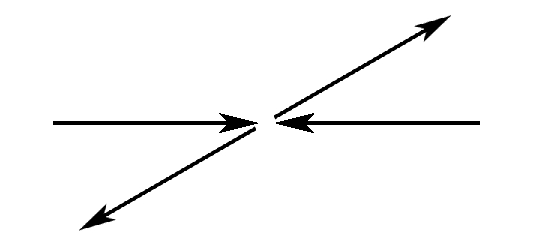
\includegraphics[width=0.55\textwidth]{figs/cms.pdf}}
\put(25,5){$p_4$}
\put(10,65){$p_1$}
\put(255,65){$p_2$}
\put(240,125){$p_3$}
\put(175,72){$\theta$}
\end{picture}
\end{center}
\caption{\label{fig:cms} Coordinate system for the center-of-mass frame.}
\end{figure}

In the center of mass frame shown in Fig.~\ref{fig:cms} the cross-section is given by:
\begin{equation}
\frac{d\sigma}{d\Omega} = \frac{1}{64\pi^2Q^2}|\mathcal{M}|^2
\end{equation}
assuming $Q^2$ is much larger than the lepton masses.

\begin{Exercise}
Show that in the center of mass frame:
\begin{eqnarray}
p_4 p_2 \; p_3 p_1 + p_4 p_1 \; p_3 p_2 +  &=& 2 E^4 \left( 1 + \cos^2 \theta \right) \label{eqn:pplus}\\
p_4 p_2 \; p_3 p_1 -  p_4 p_1 \; p_3 p_2  &=& 4 E^4 \cos \theta \label{eqn:pminus}
\end{eqnarray}
\end{Exercise}

\begin{Exercise}
From Equation~\ref{eqn:xg} and the results of this section, show that the spin-averaged differential and total cross section for the pure QED process is given by:
\begin{equation} \label{eqn:qeddsigma}
\left(\frac{d\sigma}{d\Omega}\right)_\gamma = \frac{\alpha^2}{4 Q^2}\left(1 + \cos^2\theta\right)
\end{equation}
where the fine structure constant $\alpha = e^2/4\pi$ in our units with $\hbar = c = 1$.  Also show that the spin-averaged total cross-section is:
\begin{equation} \label{eqn:qedsigma}
\sigma_\gamma = \frac{4 \pi \alpha^2}{3 Q^2}
\end{equation}
Using the numerical value in Equation~\ref{eqn:hcs}, compute the total cross-section in mbarn at $E=1~\GeV$.
Note that at this point, you have everything needed to complete the first two MadGraph exercises.
\end{Exercise}

\section{Z Boson}

For the pure $Z$ process $e^+e^- \to Z \to \mu^+\mu^-$ we saw (Equation~\ref{eqn:mz}) that the matrix element is:
\begin{equation}
\mathcal{M}_Z = \frac{ig^2}{4\cos^2\theta_W}\; \frac{1}{Q^2-m_Z^2+i\epsilon} \; \left\{ \bar{w} \gamma^\mu  (\gv-\ga\gamma_5) x \right\} \left\{ \bar{v} \gamma_\mu (\gv-\ga\gamma_5) u \right\}
\end{equation}
And so putting $A^\mu = A_Z^\mu \equiv \gamma^\mu(\gv-\ga\gamma^5)$ in Equation~\ref{eqn:maa} and recalling Equation~\ref{eqn:tildez} we obtain:
\begin{equation}
X_Z \equiv \frac{1}{4} \sum_{\rm spins} |M_Z|^2 = \frac{g^4}{64\cos^4\theta_W} \frac{1}{(Q^2-m_Z^2)^2+\epsilon^2}\Tr\left( \ps_4 \, A_Z^\mu \, \ps_3\, A_Z^\nu \right) \Tr\left( \ps_1 \, A_{Z\mu} \, \ps_2 \, A_{Z\nu} \right) \label{eqn:mzz}
\end{equation}
Where we now encounter a product of two traces, both of form:
\begin{eqnarray}
\Tr\left\{\Ps A_Z^\mu\Qs A_Z^\nu\right\} &=& \Tr\left\{\Ps\gamma^\mu(\gv-\ga\gamma_5)\Qs\gamma^\nu(\gv-\ga\gamma_5) \right\} \notag \\
&=& \gv^2 \Tr\left(\Ps\gamma^\mu\Qs\gamma^\nu\right)+\ga^2\Tr\left(\Ps\gamma^\mu\gamma^5\Qs\gamma^\nu\gamma^5\right)
-\gv\ga\left\{\Tr\left(\Ps\gamma^\mu\gamma_5\Qs\gamma^\nu\right)+\Tr\left(\Ps\gamma^\mu\Qs\gamma^\nu\gamma^5\right)\right\} \notag \\
&=& (\gv^2 + \ga^2) \Tr\left(\Ps\gamma^\mu\Qs\gamma^\nu\right)-2\gv\ga\Tr\left(\Ps\gamma^\mu\Qs\gamma^\nu\gamma^5\right) \label{eqn:trz}
\end{eqnarray}
where in the last line we have used $(\gamma_5)^2=1$, $\gamma_5\gamma^\mu=-\gamma_5\gamma^\mu$, and took care to recall that there is a $\gamma^\mu$ associated with each $\Ps$ and $\Qs$.

Equation~\ref{eqn:mzz} contains a product of the trace we have simplified in Equation~\ref{eqn:trz}.  We showed in an earlier exercise (Equation~\ref{eqn:trab})
that:
\begin{equation}
\Tr\left(\Ps\gamma^\mu\Qs\gamma^\nu\right) \Tr\left(\Rs\gamma_\mu\Ss\gamma_\nu\gamma^5\right) = 0 \label{eqn:trab}
\end{equation}
which simplifies the product, as there are there are no cross-terms.  As a result, we have from Equations~\ref{eqn:mzz} and \ref{eqn:trz}:
\begin{equation}
\begin{split}
X_Z  = \frac{g^4}{64\cos^4\theta_W} \frac{1}{(Q^2-m_Z^2)^2+\epsilon^2} \times \kern 5cm \\
\left\{ (\gv^2 + \ga^2)^2  \Tr\left( \ps_4 \, \gamma^\mu \, \ps_3\, \gamma^\nu \right) \Tr\left( \ps_1 \, \gamma_\mu \, \ps_2 \, \gamma_\nu \right)
+4\gv^2\ga^2\Tr\left( \ps_4 \, \gamma^\mu \, \ps_3\, \gamma^\nu \gamma_5\right) \Tr\left( \ps_1 \, \gamma_\mu \, \ps_2 \, \gamma_\nu \gamma_5 \right) \right\}
\end{split} \label{eqn:xzalmost}
\end{equation}

\begin{Exercise}
By applying Equations~\ref{eqn:traa},\ref{eqn:trbb},\ref{eqn:pplus} and \ref{eqn:pminus} to Equation~\ref{eqn:xzalmost} show that:
\begin{equation}
X_Z  = \frac{g^4}{16 \cos^4\theta_W} \frac{Q^4}{(Q^2-m_Z^2)^2 + \epsilon^2} \left\{ (\gv^2 + \ga^2)^2  \left(  1 + \cos^2\theta \right)
+8\gv^2\ga^2 \cos\theta \right\}
\end{equation}
\end{Exercise}

\begin{Exercise}
Show that
\begin{eqnarray}
\left(\frac{d\sigma}{d\Omega}\right)_Z &=& \frac{g^4}{1024\pi^2\cos^4\theta_W} \frac{Q^2}{(Q^2-m_Z^2)^2 + \epsilon^2} \left\{ (\gv^2 + \ga^2)^2  \left(  1 + \cos^2\theta \right)+8\gv^2\ga^2 \cos\theta \right\} \notag \\
&=& \frac{m_Z^4 G_F^2}{32\pi^2} \frac{Q^2}{(Q^2-m_Z^2)^2 + \epsilon^2} \left\{ (\gv^2 + \ga^2)^2  \left(  1 + \cos^2\theta \right)+8\gv^2\ga^2 \cos\theta \right\} \label{eqn:dsigmaz}
\end{eqnarray}
where the last form is in agreement with LEP z-pole paper Equation 1.34.  Therefore, show that:
\begin{equation}
\sigma_Z = \frac{G_F^2 m_Z^4(\gv^2 + \ga^2)^2}{6\pi} \frac{Q^2}{(Q^2-m_Z^2)^2 + \epsilon^2}
\end{equation}
Putting $\epsilon = \Gamma_Z m_Z$, and evaluating at $Q=m_Z$:
\begin{equation}
\sigma_Z  = \frac{G_F^2 m_Z^4(\gv^2 + \ga^2)^2}{6\pi\Gamma_Z^2} 
\end{equation}
\end{Exercise}

\begin{Exercise}
Evaluate the total cross-section for $e^+e- \to Z \to \mu+\mu-$ at the z-pole and compare to the LEP reported leptonic pole cross-section $\sigma_{\rm lep}^0 = 2.0003~{\rm nb}$.

%ANSWER:
%\begin{verbatim}
%>>> (1.0E6)*(0.3894)*((1.166E-5)**2)*((91.18)**4)/(6*3.1415*2.495**2)*(0.251)**2
%1.964759639120202
%\end{verbatim}
\end{Exercise}

\section{$Z$-Boson decays to hadrons}

\begin{figure}[htbp]
\begin{center}
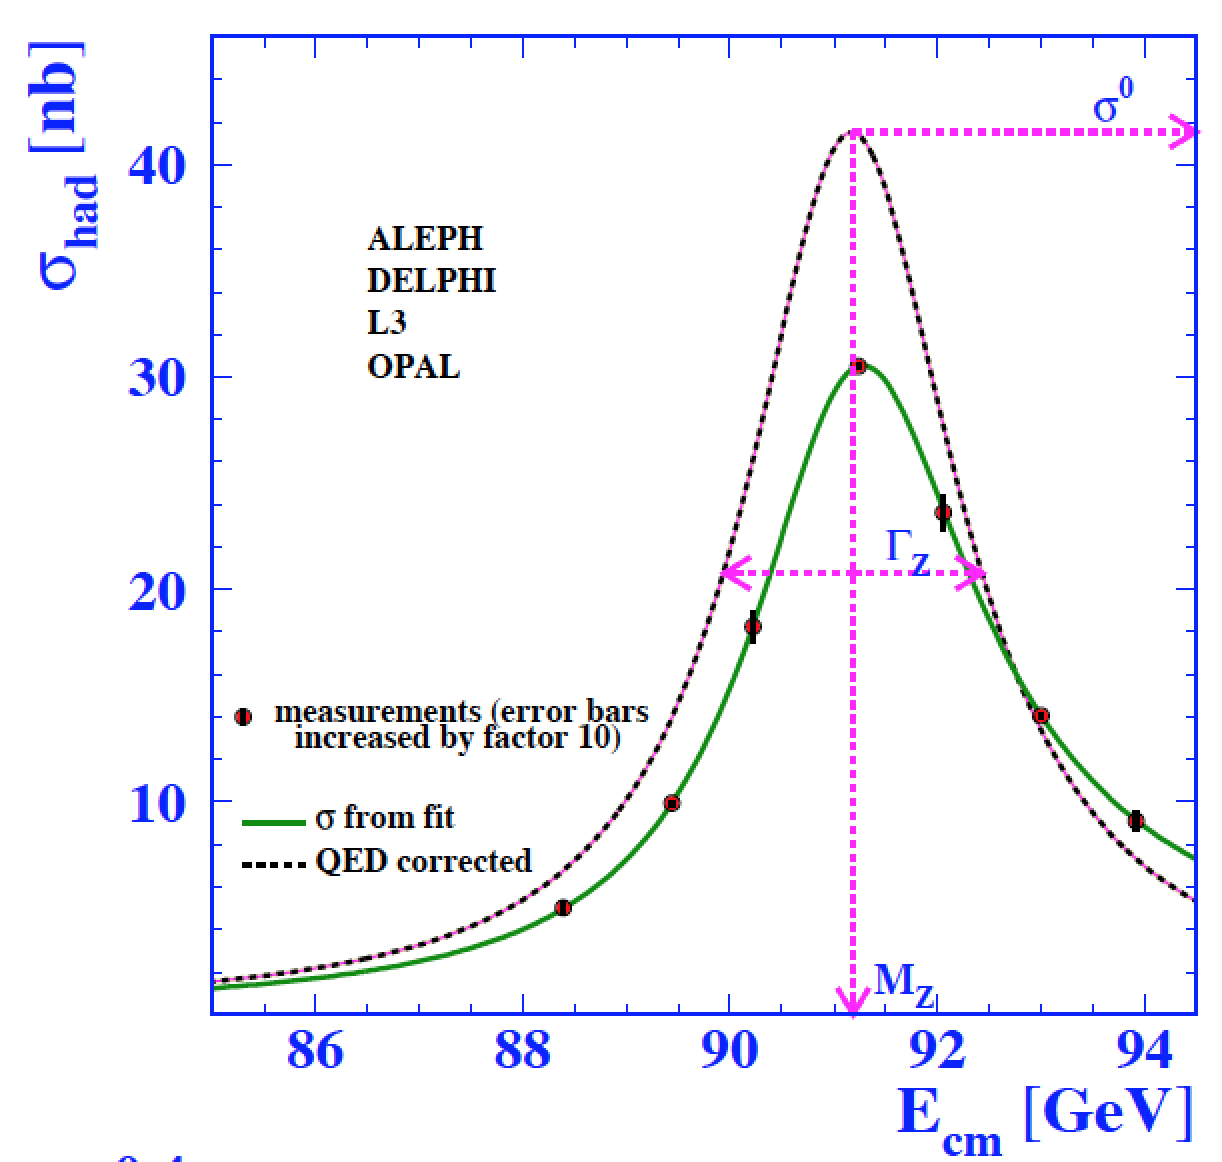
\includegraphics[width=0.55\textwidth]{figs/lep_zpeak.png}
\end{center}
\caption{\label{fig:lepzpeak} Z peak measured at LEP.}
\end{figure}

The cross-section for the process $e^+ e^- \to Z \to f \bar{f}$ proceeds much like the above, except that there are new two sets of couplings 
involved $g_{{\rm v}e}$ and $g_{{\rm a}e}$ for the electrons and $g_{{\rm v}f}$ and $g_{{\rm a}f}$ for the fermions.  For the process 
$e^+ e^- \to e^+ e^-$ one must consider both $s$ and $t$ channel processes, but we only considered the $s$-channel in our calculation and will not consider this process.  There is now a color factor $N_C$ which is 3 for quarks and 1 for leptons.  The resulting total cross-section, at the $Z$-peak, is given by:
\begin{equation}
\sigma_Z^{ff}  = \frac{G_F^2 m_Z^4}{6\pi\Gamma_Z^2}  N_C (g_{{\rm v}e}^2 + g_{\rm{a}e}^2) (g_{{\rm v}f}^2 + g_{{\rm a}f}^2)
\end{equation}

\begin{Exercise}
Calculate a numerical value and compare with the LEP reported hadronic pole cross-section $\sigma_{\rm hadron}^0=41.541~{\rm nb}$.

%ANSWER:
%\begin{verbatim}
%>>> 588.4/(6*3.1415)*3*0.2514*(2*0.2868+3*0.3696)
%39.60957087760624
%\end{verbatim}

Before LEP began it's celebrated scan of the $Z$-peak, theorist anticipated that there would be substantial radiative corrections due primarily to initial state radiation.  Intuitively, no matter how perfectly the electron and positron energies are tuned, if one of the initial state particles radiates a photon which is not detected by the experiment, the $Z$ moves off-shell.  These effects lower and broaden the $Z$ peak.  At the peak, an initial estimate for the correction reveals that a factor of about 0.72 should be applied to the total cross-section.  Multiply your answer above to obtain the actual cross-section at the peak, and compare to Fig.~\ref{fig:lepzpeak} (More sophisticated corrections yield even better agreement.  See Burgess and Moore, p 223.)

\end{Exercise}

%ANSWER:
%\begin{verbatim}
%>>> 39.61*0.72
%28.519199999999998
%\end{verbatim}

%\section{$Z$ Boson Width}
%Work in progress...
%
%\begin{Exercise}
%From $(12\pi/m_Z^2) \Gamma_{ee} \Gamma_{\mu\mu} / \Gamma_Z^2$:
%\begin{verbatim}
%\end{verbatim}
%\end{Exercise}

\section{$Z/\gamma$ Inteference}

The $Z/\gamma$ Interference term mixes $\gamma^\mu$ and $\gamma^\mu\gamma_5$.  Putting $A^\mu=\gamma^\mu$ and $B^\mu = A_Z^\mu \equiv \gamma^\mu(\gv-\ga\gamma^5)$ in Equation~\ref{eqn:mab} and recalling Equation~\ref{eqn:tildez} we obtain:
\begin{equation}
X_{Z\gamma} \equiv \frac{1}{4} \sum_{\rm spins} \mathcal{M}_\gamma^\dagger \mathcal{M}_Z = 
\frac{g^2 e^2}{16\cos^2\theta_W} \frac{1}{Q^2}\frac{1}{(Q^2-m_Z^2)+i\epsilon}\Tr\left( \ps_4 \, \gamma^\mu \, \ps_3\, A_Z^\nu \right) \Tr\left( \ps_1 \, \gamma_\mu \, \ps_2 \, A_{Z\nu} \right) \label{eqn:maz}
\end{equation}
where the traces in the product now have form:
\begin{eqnarray}
\Tr\left\{\Ps\gamma^\mu\Qs A_Z^\nu\right\} &=& \Tr\left\{\Ps\gamma^\mu\Qs\gamma^\nu(\gv-\ga\gamma_5) \right\} \notag \\
&=& \gv \Tr\left(\Ps\gamma^\mu\Qs\gamma^\nu\right)-\ga\Tr\left(\Ps\gamma^\mu\Qs\gamma^\nu\gamma^5\right)
\end{eqnarray}
\begin{Exercise}
Show that the complete interference term from $X_{Z\gamma} + X_{Z\gamma}^\dagger$ contributes:
\begin{eqnarray}
\left( \frac{d\sigma}{d\Omega} \right)_{Z\gamma} &=&  \frac{g^2 e^2}{128 \pi^2 \cos^2\theta_W} \frac{(Q^2-m_Z^2)}{(Q^2-m_Z^2)^2+\epsilon^2}\left\{ \gv^2 \left(1 + \cos^2 \theta \right) + 2 \ga^2 \cos\theta\right\} \notag \\
&=&  \frac{G_F m_Z^2}{4 \sqrt{2} \pi} \frac{(Q^2-m_Z^2)}{(Q^2-m_Z^2)^2+\epsilon^2}\left\{ \gv^2 \left(1 + \cos^2 \theta \right) + 2 \ga^2 \cos\theta\right\} \label{eqn:dsigmazg}
\end{eqnarray} 
Notice that the interference vanishes at the $Z$-pole, then changes sign.   
\end{Exercise}

\section{LEP Results}

\begin{figure}[htbp]
\begin{center}
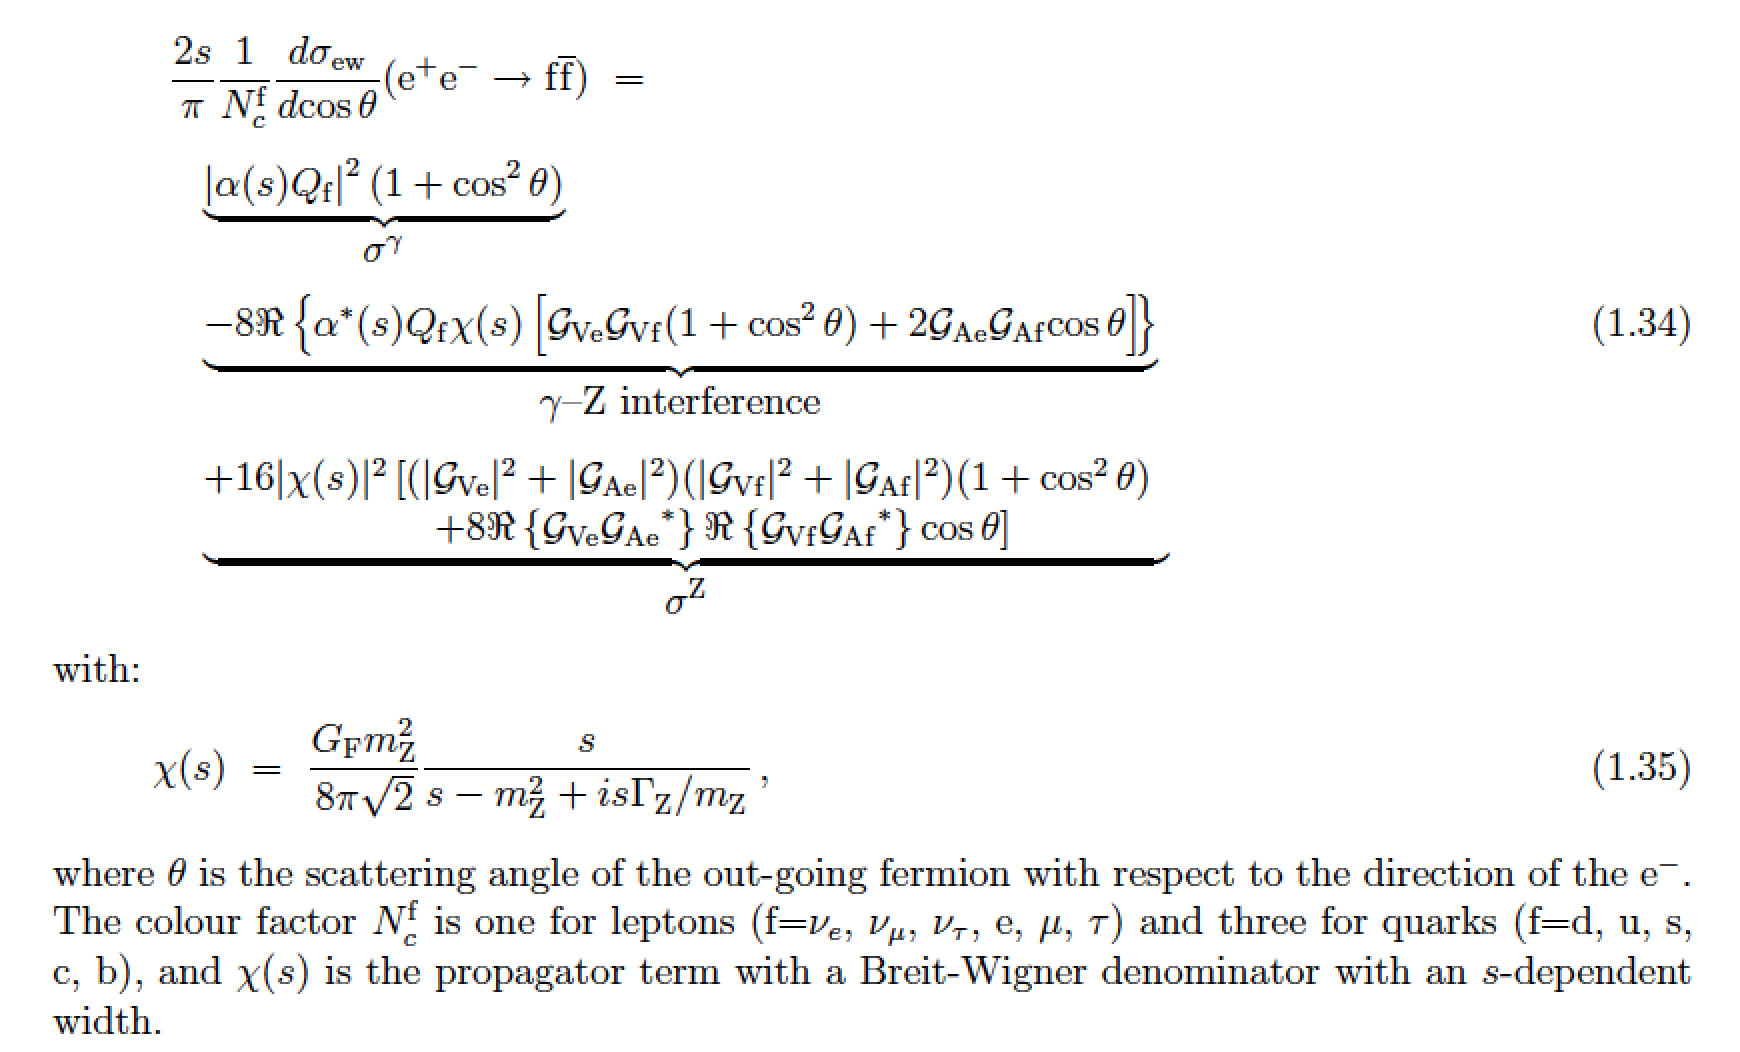
\includegraphics[width=0.90\textwidth]{figs/lep_xsec.png}
\end{center}
\caption{\label{fig:lepans} Z-cross-section from seminal LEP z-pole paper}
\end{figure}

\begin{figure}[htbp]
\begin{center}
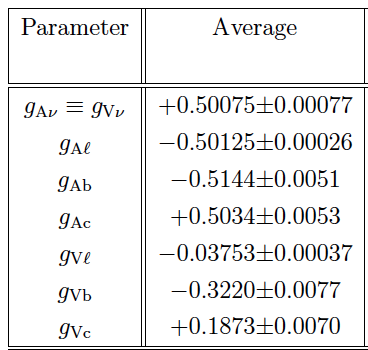
\includegraphics[width=0.40\textwidth]{figs/lep_couplings_quarks.png}
\end{center}
\caption{\label{fig:lepcouplling} Effective couplings measured at LEP.}
\end{figure}

\begin{figure}[htbp]
\begin{center}
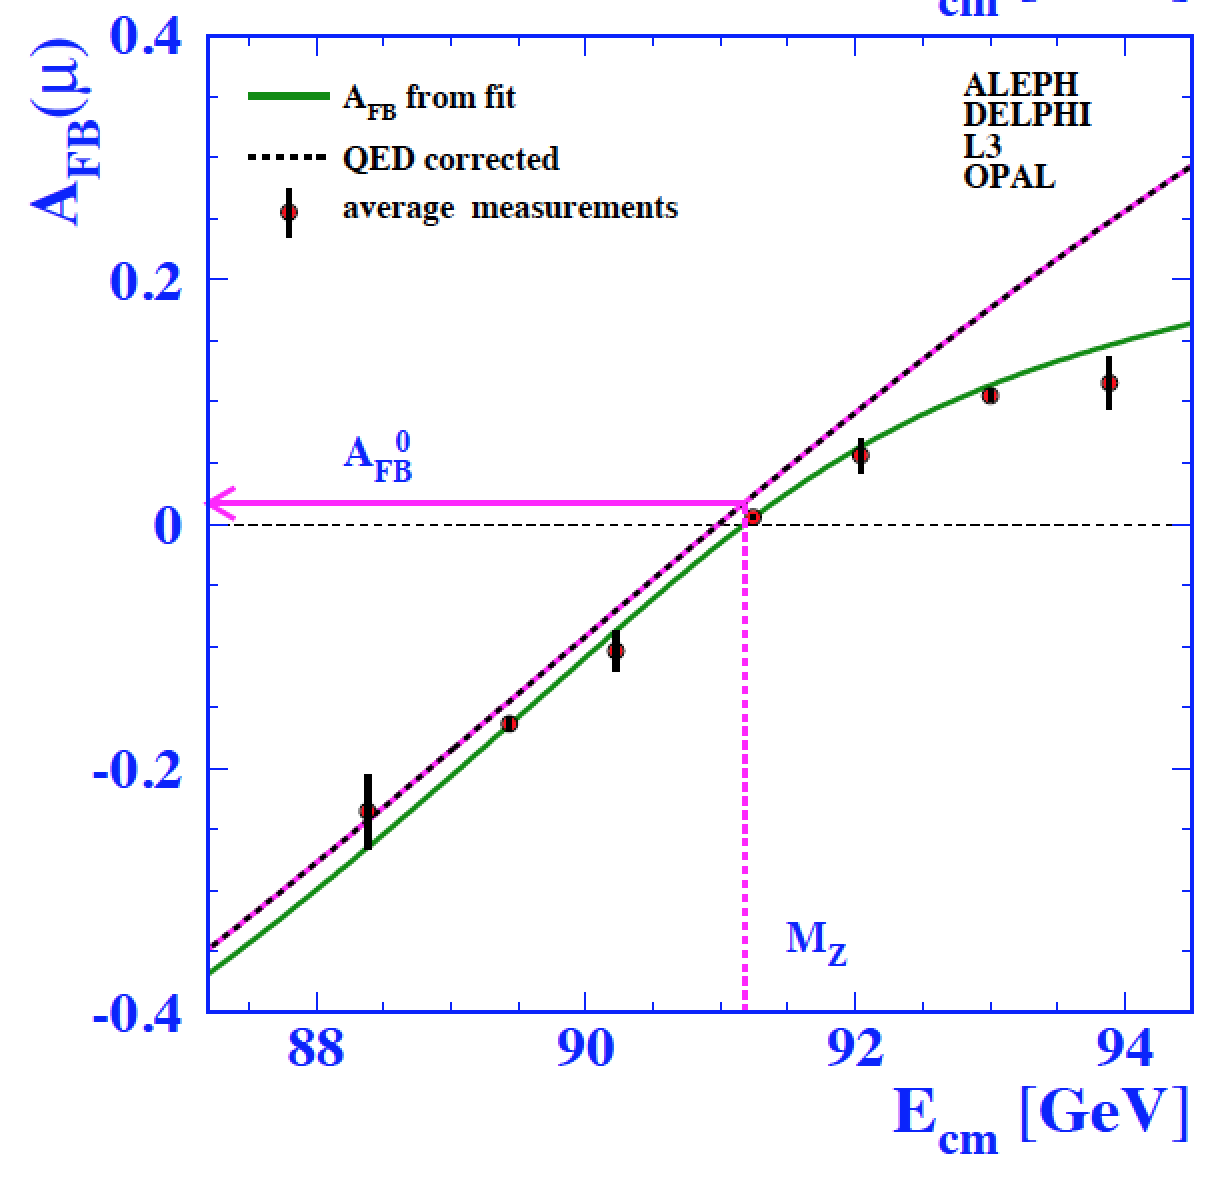
\includegraphics[width=0.55\textwidth]{figs/lep_fwbw.png}
\end{center}
\caption{\label{fig:lepfwbw} FB measured at LEP.}
\end{figure}

\section{Madgraph Exercises}

All the command prompts in these exercises assume you are running them from the main MadGraph directory.  It is assumed that ROOT is already installed.
\begin{Exercise}
Download and install Madgraph on your laptop, then run the tutorial:
\begin{verbatim}
> ./bin/mg5_aMC
MG5_aMC>tutorial
\end{verbatim}
\end{Exercise}

\begin{Exercise}
Use Madgraph to determine the total cross-section as a function of energy for the process $e^+ e^- \to Z \to \mu+ \mu-$ well below the $Z$-pole.  Plot your results and compare with Equation~\ref{eqn:qedsigma}.  For MadGraph to reproduce the theory calculation precisely you'll need to do the following:
\begin{itemize}
\item Generate the process:
\begin{verbatim}
> generate e+ e- > a > mu+ mu-
> output demo
> launch demo
\end{verbatim}
\item Set the beam energy in the file {\tt run\_card.dat}.
\item Use a consistent value for the fine structure constant, $\alpha$.  By default, MadGraph uses the value at the $Z$-pole, as set by the parameter {\tt aewm1} in the file {\tt param\_card.dat}. 
\item Reduce the parton-level cuts on $\eta$ and $p_{\rm T}$ of final state leptons.  The default values of these cuts are inefficient at center-of-mass energy below the $Z$-pole.  Change the parameters {\tt etal} and {\tt ptl} in the file {\tt run\_card.dat}.
\end{itemize}
\end{Exercise}

\begin{Exercise}
Using MadGraph, plot the differential cross-section as a function of both $\theta$ and $\cos\theta$.  Compare with Equation~\ref{eqn:qedsigma}. Don't forget the Jacobian factor for the coordinate transformation.

To generate the differential distributions, you will need access to parton four-vectors, which you can get via ExRootAnalysis.  If not already done, you can simply run the MadGraph command 
\begin{verbatim}
> install ExRootAnalysis
\end{verbatim}
This includes a utility for converting the LHE format files produced by MadGraph into the ExRootAnalysis format which you can then plot using ROOT.  For example:
\begin{verbatim}
> cp demo/Events/run_01/unweighted_events.lhe.gz .
> gunzip unweighted_events.lhe.gz .
> /ExRootAnalysis/ExRootLHE unweighted_events.lhe lhe.root
\end{verbatim}
\end{Exercise}
An example ExRootAnalysis macro to process the root file is listed in the appendix.  

\begin{Exercise}
Use Madgraph to reproduce the total hadronic cross-section as a function of energy, and compare to Fig.~\ref{fig:lepans}.
You'll need to adjust the parton-level jet cuts in order to get good agreement.  Also plot the cross-section corrected for initial and final state radiation using the simple flat factor of 0.72 discussed in the text.
% maybe check z-pole paper for appropriate parton level cuts?
\end{Exercise}

\begin{Exercise}
Use Madgraph to reproduce the total hadronic cross-section as a function of energy, and compare to Fig.~\ref{fig:lepans}.
You'll need to adjust the parton-level jet cuts in order to get good agreement.  Also plot the cross-section corrected for initial and final state radiation using the simple flat factor of 0.72 discussed in the text.
\end{Exercise}

\begin{Exercise}
Use Madgraph to plot the differential cross section wrt $\theta$ and $\cos \theta$ for the process $e^+ e^- \to \mu^+ \mu^-$ at an energy where you expect the asymmetry to be large, and compare to what you expect from your theory calculations, i.e. Equations~\ref{eqn:dsigmaz} and \ref{eqn:dsigmazg}

Measure the forward-backward asymmetry as a function of center-of-mass energy near the $Z$-pole (as in Fig.~\ref{fig:lepfwbw} and also compare with your theory predictions.

\end{Exercise}


\newpage

\appendix

\section{Analysis Code Example}
An example ExRootAnalysis macro to process the root file and access parton-level four-vectors.  You'll need to point ROOT to two libraries, libPhysics, which should be included with your ROOT installation, and libExRootAnalysis, which should be in the {\tt ExRootAnalysis} subdirectory from your main MadGraph directory.

\begin{verbatim}
demo(){
  //setup a rootlogon.C file to do this, or do it here, but you may need full path:
  //gSystem->Load("libExRootAnalysis.dylib");
  //gSystem->Load("libPhysics");

  TChain chain("LHEF");
  chain.Add("lhe.root");
  ExRootTreeReader *treeReader = new ExRootTreeReader(&chain);
  Long64_t numberOfEntries = treeReader->GetEntries();

  TClonesArray *branchGen = treeReader->UseBranch("Particle");  

  for(Long64_t entry = 0; entry < numberOfEntries; ++entry){
    treeReader->ReadEntry(entry);
    int ngen = branchGen->GetEntries();
    for (int i=0; i<ngen; i++){
      TRootGenParticle * part = (TRootGenParticle*) branchGen->At(i);
      int pid = part->PID;

      // in my install, there is a little bug, which this remapping corrects:
      double px = part->E;
      double py = part->Px;
      double pz = part->Py;
      double e  = part->Pz;

      cout << pid << ":  px=" << px << ", py=" << py;
      cout << ", pz=" << pz << ", e=" << e << "\n";
    }
    if (entry>5) break;
  }
}
\end{verbatim}

\newpage

\section{Physical and Couplings Constants}

Properties of the $Z$ boson:
\begin{eqnarray*}
m_Z &=& 91.19~\GeV \\
\Gamma_Z &=& 2.495~\GeV \\
{\rm Br}(Z \to \ell \ell) &=& 3.363\% \\
{\rm Br}(Z \to {\rm hadrons}) &=& 69.91\%
\end{eqnarray*}

We use the convention that $\hbar = c = 1$.  To calculate numerical values, it is generally helpful to have:
\begin{eqnarray}
(\hbar c)^2 &=& 0.3894~{\rm mbarn}\,\GeV^2 \label{eqn:hcs}\\
G_F/(\hbar c)^3 &=& 1.166\times10^{-5}~\GeV^{-2} \notag \\
G_F m_Z^2/(\hbar c)^3 &=& 0.09699 \notag \\
\frac{G_F^2 m_Z^4}{\Gamma_Z^2}(\hbar c)^2 &=& 588.4~{\rm nb} \notag 
\end{eqnarray}

The vector and axial vector couplings of the weak interaction are given, at tree-level, by:
\begin{eqnarray*}
\gv &=& T_3 - 2 Q \sin^2\theta_W\\
\ga &=& T_3
\end{eqnarray*}
where $T_3$ is the third component of weak isospin, $Q$ is the fermion charge in units of $e$, and the weak mixing angle:
\begin{equation}
\sin^2 \theta_W = 0.23120
\end{equation}
is the best estimate at $m_Z$.  The resulting couplings by each Fermion type are listed in Table~\ref{tbl:gva}:
\begin{table}[htbp]
\begin{center}
\caption{ \label{tbl:gva} The Fermion neutral-current coupling constants.}
\begin{tabular}{lrrrrrr}
Fermion & $T_3$ & $Q$ & $\gv$ & $\ga$ & $\gv^2 + \ga^2$  & $\gv\ga$\\
$\nu_e$,$\nu_\mu$,$\nu_\tau$ & $+\frac{1}{2}$ &0 &  0.5 & 0.5 & 0.5 & 0.25\\
$e$,$\mu$,$\tau$ & $-\frac{1}{2}$ & -1                     & -0.5 &  -0.03760 & 0.2514 & 0.01880\\
$u$,$c$,$t$ &  $+\frac{1}{2}$ &  $+\frac{2}{3}$ &  0.5 &  0.19173 &  0.2868 & 0.09587\\
$d$,$s$,$b$ &  $-\frac{1}{2}$ &  $-\frac{1}{3}$ &  -0.5 &  -0.3459 &  0.3696 & 0.1729\\
\end{tabular}
\end{center}
\end{table}

The weak coupling parameter $g$ is related to Fermi's constant by:
\begin{displaymath}
\frac{G_F}{\sqrt{2}}=\frac{g^2}{8m_W^2}(1+\Delta r)
\end{displaymath}
where we will take the radiative corrections $\Delta r = 0$.

The electric and weak coupling are related by:
\begin{displaymath}
e = g \sin \theta_W
\end{displaymath}

The mass of the weak bosons and $\theta_W$ are related by:
\begin{displaymath}
 \rho_0 =  \frac{m_W^2}{m_Z^2\cos^2\theta_W^2} 
\end{displaymath}
where $\rho_0 = 1$ in the Standard Model.

In our units we have:
\begin{displaymath}
 \alpha = e^2 / 4 \pi 
\end{displaymath}
due to running of this constant, at the $z$-pole we have:
\begin{displaymath}
1/\alpha = 127.9
\end{displaymath}
while at low energy
\begin{displaymath}
1/\alpha = 137.0
\end{displaymath}



\end{document}




